\begin{figure}[t]
\centering
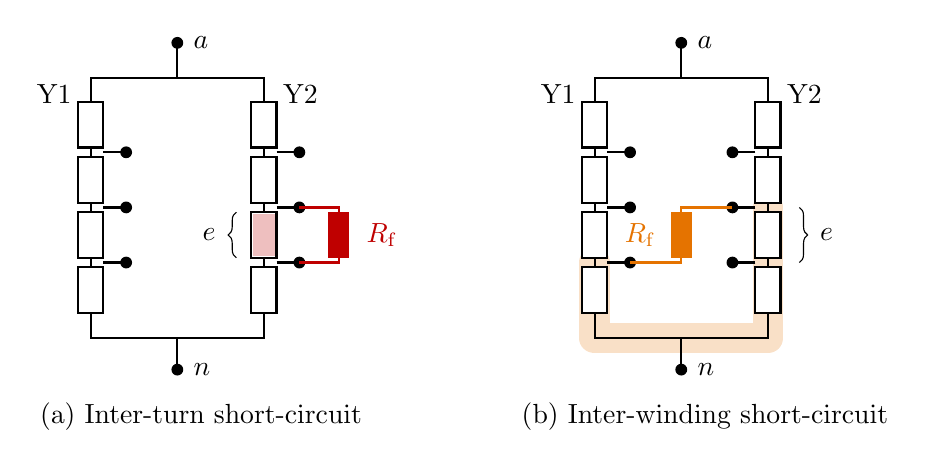
\begin{tikzpicture}[
  font=\normalsize, x=1cm, y=1cm,
  wire/.style={thick},
  coil/.style={draw, thick, fill=white, minimum width=3.2mm, minimum height=5.8mm, inner sep=0},
  tap/.style={circle, fill=black, inner sep=0, minimum size=1.5mm},
  rf/.style={draw, thick, fill=white, minimum width=2.4mm, minimum height=5.5mm, inner sep=0},
  it/.style={red!75!black},
  iw/.style={orange!90!black}
]
%% One phase (a--n) of the double-star stator: two parallel branches Y1 and Y2 of four coil groups with
%% tapped derivation points. Panel (a) inter-turn fault, panel (b) inter-winding fault.
\foreach \dx in {0, 6.4} {
  % circulating path of the inter-winding fault (panel b only), drawn first so that it lies behind
  \ifdim \dx pt > 1pt
    \draw[iw, line width=11pt, line cap=round, line join=round, opacity=0.22]
      (\dx+0.9,1.71) -- (\dx+0.9,0.75) -- (\dx+3.1,0.75) -- (\dx+3.1,2.41);
  \fi
  % terminal, junctions, branches, neutral
  \node[tap, label={right:$a$}] at (\dx+2.0,4.5) {};
  \draw[wire] (\dx+2.0,4.5) -- (\dx+2.0,4.05) -- (\dx+0.9,4.05) -- (\dx+0.9,0.75) -- (\dx+2.0,0.75) -- (\dx+2.0,0.35);
  \draw[wire] (\dx+2.0,4.05) -- (\dx+3.1,4.05) -- (\dx+3.1,0.75) -- (\dx+2.0,0.75);
  \node[tap, label={right:$n$}] at (\dx+2.0,0.35) {};
  \node[anchor=east] at (\dx+0.78,3.85) {Y1};
  \node[anchor=west] at (\dx+3.22,3.85) {Y2};
  \foreach \bx in {0.9, 3.1} {
    \foreach \cy in {3.46, 2.76, 2.06, 1.36} { \node[coil] at (\dx+\bx,\cy) {}; }
  }
  % taps of Y1 point into the gap between the branches
  \foreach \ty in {3.11, 2.41, 1.71} {
    \draw[wire] (\dx+1.06,\ty) -- (\dx+1.35,\ty); \node[tap] at (\dx+1.35,\ty) {};
  }
}
%% (a) inter-turn: two taps of one branch (Y2) shorted through R_f; the shorted coil group is shaded
\begin{scope}
  \foreach \ty in {3.11, 2.41, 1.71} {
    \draw[wire] (3.26,\ty) -- (3.55,\ty); \node[tap] at (3.55,\ty) {};
  }
  \fill[it, opacity=0.25] (2.96,2.33) rectangle (3.24,1.79);
  \draw[it, thick] (3.55,2.41) -- (4.05,2.41) -- (4.05,1.71) -- (3.55,1.71);
  \node[rf, it] at (4.05,2.06) {};
  \node[it, anchor=west] at (4.28,2.06) {$R_{\mathrm{f}}$};
  \draw[decorate, decoration={brace, amplitude=3pt}] (2.75,1.77) -- (2.75,2.35) node[midway, left=4pt] {$e$};
  \node at (2.3,-0.25) {(a) Inter-turn short-circuit};
\end{scope}
%% (b) inter-winding: a tap of Y1 and a tap of Y2 at different positions shorted through R_f;
%% the fault current circulates through the lower parts of both branches and the neutral link
\begin{scope}[shift={(6.4,0)}]
  \foreach \ty in {3.11, 2.41, 1.71} {
    \draw[wire] (2.94,\ty) -- (2.65,\ty); \node[tap] at (2.65,\ty) {};
  }
  \draw[iw, thick] (1.35,1.71) -- (2.0,1.71) -- (2.0,2.41) -- (2.65,2.41);
  \node[rf, iw] at (2.0,2.06) {};
  \node[iw, anchor=east] at (1.8,2.06) {$R_{\mathrm{f}}$};
  \draw[decorate, decoration={brace, mirror, amplitude=3pt}] (3.5,1.71) -- (3.5,2.41) node[midway, right=4pt] {$e$};
  \node at (2.3,-0.25) {(b) Inter-winding short-circuit};
\end{scope}
\end{tikzpicture}
\caption{Inter-turn (\textbf{a}) and inter-winding (\textbf{b}) short-circuits through $R_{\mathrm{f}}$ between taps of one phase of the double-star stator (schematic); $e$ is the fraction of a branch between the taps}\label{fig:faults}
\end{figure}
